Qt for Python (PySide2) are the official bindings for Qt 5 C++ API, provided by the Qt company. There are two main methods of using Qt in Python: the more common "Widgets" framework and Qt Quick which uses a markup language called QML. We have built our application using Widgets for a number of reasons: 
\begin{itemize}
\item Widgets feel more pythonic than Qt-Quick.
\item Widgets look more native to the OS running them.
\item Widget-based applications can be more easily tested with \texttt{pytest-qt}.
\item It easier to achieve a greater separation between interface-logic and business-logic (in our opinion).
\end{itemize}

One downside is that QML is better-suited for scaling on high-resolution displays but overall we feel that Widgets is a better fit for the requirements of the NeXus Constructor.

\begin{wrapfigure}{L}{0.4\linewidth}
\begin{center}
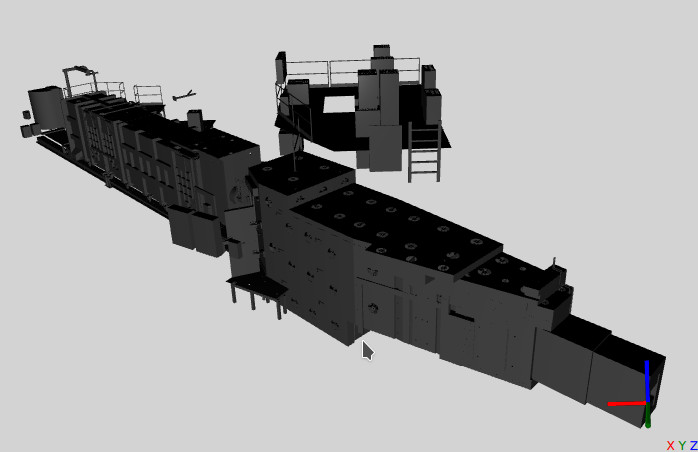
\includegraphics[width=\linewidth]{zoom.jpg}
\end{center}
\caption{The ISIS Zoom instrument in Qt3D}
\end{wrapfigure}

Qt3D provides a high-level interface to OpenGL which allows us to display instrument components in 3D. Qt3D's entity framework is similar to other GUI frameworks and 3D engines such as Unity. This means all the textures, meshes, and transformations can be stored with a single entity in the Qt3D view. An important requirement of the NeXus Constructor is a feature for handling component transformations. With Qt3D we can easily facilitate these changes without having to rebuild the entire entity from scratch.

\vspace{1.8cm}
